%%%%%%%%%%%%%%%%%%%%%%%%%%%%%%%%%%%%%%%%%%%%%%%%%%%
%% P3: Phenomenology of Particle Physics                         
%%
%% Author:  André Rubbia                   		 
%%
%% Figure 23.6 Decay energy distribution for $\mu^-\rightarrow e^-\bar\nu_e\nu_\mu$.
%%
%% This work is licensed under the Creative Commons Attribution 4.0 International License. 
%% To view a copy of this license, visit http://creativecommons.org/licenses/by/4.0/ or 
%% send a letter to Creative Commons, PO Box 1866, Mountain View, CA 94042, USA.
%%
%%%%%%%%%%%%%%%%%%%%%%%%%%%%%%%%%%%%%%%%%%%%%%%%%%%

\documentclass[a4paper,10pt]{article}

\usepackage[T1]{fontenc}
\usepackage[utf8]{inputenc}
\usepackage{lmodern}
\usepackage[labelfont=bf]{caption}
\usepackage{upgreek}

\usepackage{tikz}
\usepackage{pgfplots}
\pgfplotsset{compat=1.17}
\usepgfplotslibrary{ternary}
\usepgfplotslibrary{fillbetween}
\usepgfplotslibrary{external}

\def\d{\mathrm{d}}
\setlength{\oddsidemargin}{-1.0cm}
\setlength{\evensidemargin}{-1.0cm}
\setlength{\textheight}{25cm}
\setlength{\textwidth}{18cm}

\begin{document}

%%%%%%%%%%%%%%%%   FIGURE  %%%%%%%%%%%%%%%%%%%%%%%%%%%%%%
%%%%%%%%%%%%%%%%   FIGURE  %%%%%%%%%%%%%%%%%%%%%%%%%%%%%%
\begin{figure}[htb]
\begin{center}
%\vspace{-0.3cm}
\begin{tikzpicture}[scale=1.]
\begin{axis}[xmin=0, xmax=1,
	xtick={0,0.5,1},
%	ytick={0,1,2},
	ymin=-1, ymax=2.5,
	xlabel=Reduced energy $x$,
	ylabel=Differential decay rate,
	xmajorgrids=true,
	ymajorgrids=true,
	legend entries={$n(x)$,$n'(x)$,$\alpha(x)$},
	legend pos = outer north east]
	\addplot[domain=0:1,blue,very thick] {2*x^2*(3-2*x)};
	\addplot[domain=0:1,magenta,dashed,very thick] {12*x^2*(1-x)};
	\addplot[domain=0:1,red,dotted,very thick] {(1-2*x)/(3-2*x)};
\end{axis}
\end{tikzpicture}
\caption{Decay energy distribution for $\mu^-\rightarrow e^-\bar\nu_e\nu_\mu$.
$n(x)$ is the energy distribution for the electron (neglecting its rest mass) and
$n'(x)$ is the energy distribution of the electron antineutrino.
$\alpha(x)$ is the asymmetry parameter of the
muon (see Section~23.7 of the book).}
\end{center}
\end{figure}
%
%%%%%%%%%%%%%%%%   END FIGURE  %%%%%%%%%%%%%%%%%%%%%%%%%%%%%%
%
\end{document}
